\chapter{Vortex connections across topological interfaces}\label{chap: spin-2}
In this chapter, we both analytically and numerically investigate the physics
of topological defects when connected across topological interfaces in spin-2
Bose-Einstein condensates.
We demonstrate that a particularly rich phenomenology of topological defects
at the coherent
interface between regions of different broken symmetries can be realised in
spin-2 Bose-Einstein condensates.
In particular, we propose that an interface between uniaxial and biaxial nematic
phases exhibiting continuous and discrete order-parameter symmetry,
respectively, can be realised using existing experimental techniques.
We construct spinor wave functions that represent topological defects connecting
across the interface.
By numerical energy relaxation as well as simulations of dynamics, we
characterise the emergence of non-trivial defect core structures.
We further demonstrate the emergence of composite vortex-core structures and
continuous connection of fractional vortices representing non-Abelian charges in
interfaces involving the cyclic and ferromagnetic phases, which could be
realised through manipulation of the inter-atomic interactions.
Our results suggest the spin-2 Bose-Einstein condensates as experimentally
accessible test beds for interface physics with all combinations of continuous
and discrete symmetries, as well as phases supporting non-Abelian defects.

\section{Introduction to topological interfaces}
When topologically distinct phases, described by different order parameters,
coexist in a continuous and coherent ordered medium, a topological interface
must form at the phase boundary, where the different broken symmetries connect
smoothly.
Such interfaces are ubiquitous across many areas of physics, from the
\(A\)--\(B\) phase boundary in superfluid
helium~\cite{Salomaa1987, Volovik2009, Finne2006}, to appearing as the
termination points of cosmic strings in theories of the early
universe~\cite{Kibble1976, Vilenkin1994}, and even in brane-inflation
models in superstring theory~\cite{Dvali1999, Sarangi2002}.
They may also play an important role for superconducting materials in
solid-state physics~\cite{Bert2011}.
The different order-parameter symmetries imply that the bulk medium on either
side of the interface supports different families of topological defects and
textures, which therefore cannot cross the interface unchanged, but must either
terminate, or connect continuously and non-trivially to an object representing
the different topology on the other side.
Due to the ubiquitous nature of topological interfaces, their study in
controlled experiments becomes of general importance, inspiring the use of
laboratory systems as emulators for interface physics in contexts otherwise not
amenable to experimental observations, for example the simulation of
brane-collision processes using superfluid \(^3\)He~\cite{Bradley2007}.

Topological-interface physics becomes especially intriguing when the medium on
either or both sides of the interface exhibits point-group order-parameter
symmetry~\cite{Xiao2022}, leading to the existence of non-Abelian defects,
whose charges depend on the presence of other defects in the system and whose
dynamics is highly constrained~\cite{Poenaru1977,Mermin1979,Kobayashi2009}.
Such fully discrete order-parameters symmetries readily arise in particular
phases of spin-2 and -3 Bose-Einstein condensates
(BECs)~\cite{Barnett2006,Barnett2007,Semenoff2007,Makela2007,Yip2007,
    Kobayashi2009,Borgh2016b,Xiao2022}, which have consequently been proposed, e.g.,
as candidates for quantum-computation applications~\cite{Mawson2019} and for
realisation of non-Abelian quantum turbulence~\cite{Mawson2015}.
Spinor BECs~\cite{Kawaguchi2012,StamperKurn2013} are constructed in all-optical
traps such that the internal spin-degrees of freedom are not frozen out by
strong magnetic fields~\cite{StamperKurn1998} and provide an ideal
testing ground for investigating interface
physics~\cite{Borgh2012,Borgh2013,Borgh2014}.
Their rich phase diagrams~\cite{Kawaguchi2012} exhibit a rich variety of
phases with different order-parameter symmetries, supporting radically different
families of topological defects, such as singular
vortices~\cite{Yip1999,Isoshima2002,
    Zhou2003,Ji2008,Takahashi2009,Lovegrove2012,Weiss2019,Xiao2021}, including
vortices carrying fractional circulation~\cite{Leonhardt2000,Ji2008,Seo2015,
    Semenoff2007,Borgh2016b,Xiao2022}, and non-singular
textures~\cite{MizushimaPRL2002, MizushimaPRA2002,
    Martikainen2002,Choi2012,Lovegrove2014},
monopoles~\cite{Pietila2009,Ollikainen2017,Ruostekoski2003,Ray2014,Ray2015,
    Mithun2022}, and even Skyrmions~\cite{Tiurev2018,Lee2018} and
knots~\cite{Hall2016}.

With spin-2 BECs being experimentally readily realisable~\cite{Schmaljohann2004}
and  experimental techniques for controlled creation of vortices with internal
point-group symmetries having recently been developed~\cite{Xiao2022}, these
systems are poised as immediate candidates for the realisation of topological
interfaces with non-Abelian defect physics. Here we analytically construct spinor
wave functions representing continuous defect connections across all
permutations of topological interfaces between the different ground-state
phases of spin-2 BECs and demonstrate their energy relaxation by numerical
simulation for illustrative examples. We have previously suggested that
topological interface could be realised in spin-1 BECs through the spatial
engineering of induced Zeeman shifts~\cite{Borgh2014} (which can also control
the defect-core symmetry properties~\cite{Borgh2016a,Underwood2020}) or, less
straightforwardly, using optical or microwave Feshbach resonances to manipulate
atomic scattering lengths~\cite{Borgh2012,Borgh2013}. Here we show how the
former technique readily lends itself to the formation of a topological
interface between uniaxial (UN) and biaxial nematic (BN) phases with commonly
used atomic species such as \({87}\)Rb. We construct solutions corresponding to
connecting singly quantized and spin vortices, as well as terminating vortices.
\textcolor{red}{[Something more here]}

\section{Interface crossing solutions in a spin-2 BEC}
As discussed in Chapter~\ref{chap: ground-states}, the spin-2 BEC gives rise to
three ground state phases in the absence of a magnetic field: Ferromagnetic,
nematic, and cyclic.
In addition to these states, additional steady-state solutions that arise in
the presence of Zeeman shifts~\cite{Kawaguchi2012}.
Here, we derive a subset of the stationary solutions that offer interpolating
solutions between different ground states.

Stationary solutions of the spin-2 GPEs are obtained by substituting
\(\psi_m = \sqrt{n}\zeta_m e^{-i\mu t/\hbar}\) into
Eqs.~\eqref{eq: spin-2-GPEs-pm2}-\eqref{eq: spin-2-GPEs-0}.
Ignoring the kinetic energy term and taking \(V(\vb{r}) = 0\), this results
in
\begin{align}
    \mu\zeta_2    & = \left(-2p + 4q + c_0n +2c_1nf_z\right)\zeta_2
    + c_1nf_-\zeta_1 + \frac{c_2}{\sqrt{5}}na_{00}\zeta^*_{-2},            \\
    \mu\zeta_1    & = \left(-p + q + c_0n +c_1nf_z\right)\zeta_1
    + c_1\left(\frac{\sqrt{6}}{2}nf_-\zeta_0 +nf_+\zeta_2\right)
    - \frac{c_2}{\sqrt{5}}na_{00}\zeta^*_{-1},                             \\
    \mu\zeta_0    & = c_0n\zeta_0 + \frac{\sqrt{6}}{2}c_1\left(nf_+\zeta_1
    + nf_-\zeta_{-1}\right) + \frac{c_2}{\sqrt{5}}na_{00}\zeta_0^*,        \\
    \mu\zeta_{-1} & = \left(p + q + c_0n - c_1nf_z\right)\zeta_{-1}
    + c_1\left(\frac{\sqrt{6}}{2}nf_+\zeta_0 +nf_-\zeta_{-2}\right)
    - \frac{c_2}{\sqrt{5}}na_{00}\zeta^*_{1},                              \\
    \mu\zeta_{-2} & = \left(2p + 4q + c_0n - 2c_1nf_z\right)\zeta_{-2}
    + c_1nf_+\zeta_{-1} + \frac{c_2}{\sqrt{5}}na_{00}\zeta^*_{2}.          \\
\end{align}

We can choose the overall phase such that \(\zeta_0\) is real.
In addition, since the system is assumed to be symmetric about the \(z\)-axis,
we can let \(f_y=0\) without loss of generality.
\textcolor{red}{Need to convince myself on this last assumption.}
We consider the specific case where the transverse magnetisation is zero
\(f_{\pm} = 0\), which is valid for \(q < 0\)
Assuming the above, the stationary equations can be transformed into the
following simplified set of equations:
\begin{align}
    0 & = (-2p + 4q + c_0n + 2c_1nf_z - \mu)\zeta_2
    + \frac{c_2}{\sqrt{5}}na_{00}\zeta^*_{-2},
    \label{eq: spin-2-stationary-zeta2}                                 \\
    0 & = (2p + 4q + c_0n - 2c_1nf_z - \mu)\zeta_{-2}
    + \frac{c_2}{\sqrt{5}}na^*_{00}\zeta_{2},
    \label{eq: spin-2-stationary-zetam2}                                \\
    0 & = (-p + q + c_0n + c_1nf_z - \mu)\zeta_1
    + \frac{c_2}{\sqrt{5}}na_{00}\zeta^*_{-1},
    \label{eq: spin-2-stationary-zeta1}                                 \\
    0 & = (p + q + c_0n - c_1nf_z - \mu)\zeta_{-1}
    + \frac{c_2}{\sqrt{5}}na^*_{00}\zeta_1,
    \label{eq: spin-2-stationary-zetam1}                                \\
    0 & = \left(c_0n + \frac{c_2}{\sqrt{5}}na_{00} - \mu\right)\zeta_0.
    \label{eq: spin-2-stationary-zeta0}
\end{align}

Noting that the above equations are decoupled in three parts, we can construct
the following matrix equations relating to
Eqs.~\eqref{eq: spin-2-stationary-zeta2}-\eqref{eq: spin-2-stationary-zetam2}
and Eqs.~\eqref{eq: spin-2-stationary-zeta1}
-~\eqref{eq: spin-2-stationary-zetam1}, respectively, as
\begin{align}
    \mqty(4q + 2\beta -\tilde{\mu} & \alpha                           \\
    \alpha^*                       & 4q - 2\beta -\tilde{\mu})
    \mqty(\zeta_2                                                     \\
    \zeta_{-2}^*)                  & = 0, \label{eq: zeta-pm2-matrix} \\
    \mqty(q + \beta -\tilde{\mu}   & -\alpha                          \\
    -\alpha^*                      & q - \beta -\tilde{\mu})
    \mqty(\zeta_1                                                     \\
    \zeta_{-1}^*)                  & = 0, \label{eq: zeta-pm1-matrix}
\end{align}
with Eq.~\eqref{eq: spin-2-stationary-zeta0} being recast as
\begin{equation}\label{eq: spin-2-stationary-zeta0-recast}
    (\alpha - \tilde{\mu})\zeta_0 = 0.
\end{equation}
Here, \(\tilde{\mu} = \mu - c_0n\), \(\alpha = c_2na_{20}/\sqrt{5}\) and
\(\beta = c_1nf_z - p\).
The stationary solutions are then classified according to the determinant of
the coefficient matrices of the above equations.
Explicitly, these are
\begin{align}
    D_2 & = {(4q-\tilde{\mu})}^2 -4\beta^2 - |\alpha|^2, \label{eq: D2}  \\
    D_1 & = {(q - \tilde{\mu})}^2 - \beta^2 - |\alpha|^2. \label{eq: D1}
\end{align}
From these determinants and Eq.~\eqref{eq: spin-2-stationary-zeta0-recast},
we can derive stationary solutions that interpolate between different ground
states of the spin-2 system.

\subsection{Ferromagnetic to biaxial nematic}
Consider the case \(D_1 \neq 0\) and \(D_2 = 0\).
If \(D_1 \neq 0\), then Eq.~\eqref{eq: D1} implies \(\zeta_1=\zeta_{-1} = 0\).
Additionally, if \(\alpha \neq \tilde{\mu}\),
then Eq.~\eqref{eq: spin-2-stationary-zeta0-recast} implies \(\zeta_0 = 0\).
\textcolor{red}{Rest of derivation here.}

The resulting stationary solution has the form
\begin{equation}\label{eq: FM-BN-interpolating-spinor}
    \zeta_\mathrm{FM-BN} = \mqty(\sqrt{\frac{1 + f_z/2}{2}} \\ 0 \\ 0 \\ 0 \\
    \sqrt{\frac{1 - f_z/2}{2}}),
\end{equation}
where \(f_z = p / [(c_1-c_2/20)n]\) gives the longitudinal magnetisation.
One can see that at \(p = \pm 2(c_1-c_2/20)n\) the above solution becomes
the ferromagnetic state with spin \(f_z = \pm 2\).
Alternatively, the solution becomes the BN state when \(p=0\).
Therefore, this spinor provides an interpolating solution between the
ferromagnetic and BN phases, which is controlled by the linear Zeeman shift,
\(p\).

Defect states that span the interface can be constructed from the steady state
solutions by applying a condensate phase \(\phi \) and spin rotation defined by
Euler angles (\(\alpha, \beta, \gamma \))
[see Eq.~\eqref{eq: spin-2-rotation-matrix}].
In this Chapter we focus only on a small subset of the possible defects present
in the spin-2 system.

We start from the interpolating spinor between the FM and BN phases in
Eq.~\eqref{eq: FM-BN-interpolating-spinor}.
The simplest vortex case to consider is that of a singular, singly quantised
vortex (SQV) on both sides of the interface.
Such a vortex is formed of a \(2\pi \) winding of the condensate phase about
the vortex core.
This winding is achieved by letting \(\phi = \varphi \), where \(\varphi \) is
the azimuthal angle about the core and letting the Euler angles be constant.
This resulting interpolating spinor then reads
\begin{equation}
    \zeta_\mathrm{FM-BN}^\mathrm{SQV} =
    \mqty(e^{i\varphi}\sqrt{\frac{1 + f_z/2}{2}} \\ 0 \\ 0 \\ 0 \\
    e^{i\varphi}\sqrt{\frac{1 - f_z/2}{2}}),
\end{equation}
where we have taken \(\alpha=\beta=\gamma=0\) for simplicity.
Despite being characterised by the same phase winding on both sides of the
interface, each SQV represents an entirely different object due to the
differing topologies on either side.

Another solution connecting different vortex states can be obtained from the
above by removing the winding from one of the \(\zeta_{\pm 2}\) components.
For example, if \(f_z\) interpolates from \(f_z=0\) to \(f_z=2\) and the winding
was removed from the \(\zeta_{-2}\) component, this solution would then connect
an SQV on the FM side to a half-quantum vortex (HQV) on the BN side.
For that same state, if the winding was instead removed from the \(\zeta_{2}\)
component, then the HQV on the BN side would continuously connect to a
vortex-free state on the FM side.

Spinor BECs support the non-dissipative flow of condensate spin, which gives
rise to vortex structures that carry a spin circulation, referred to as a spin
vortex.
Such vortices arise in all phases of the spin-2 BEC [REF].
An interpolating solution involving a spin vortex can be constructed through the
choice of \(\varphi=\gamma=0\) and \(\alpha=\varphi/2\) which results in a
singular SQV on the FM side which connecting to a BN spin vortex.
The resulting spinor reads
\begin{equation}
    \zeta_\mathrm{FM-BN}^\mathrm{SQV-SV} =
    \mqty(e^{-i\varphi}\sqrt{\frac{1 + f_z/2}{2}} \\ 0 \\ 0 \\ 0 \\
    e^{i\varphi}\sqrt{\frac{1 - f_z/2}{2}}),
\end{equation}
where we have chosen \(\beta = 0\).

As seen in Sec.~\ref{sec: vortices-spin-1}, the FM phase of a spin-1 BEC can
host a non-singular, coreless vortex that has a characteristic fountain-like
spin texture.
A coreless vortex can also be constructed in the spin-2 system following a
similar procedure and having \(\beta=\beta(\rho)\) be a monotonically increasing
function of the radial coordinate \(\rho = \sqrt{x^2 + y^2}\).
This, in addition to choosing the Euler angles
\(\phi - 2\gamma = 2\alpha = 2\varphi \) leads to the interpolating spinor
(\(\gamma=0\))
\begin{equation}\label{eq: FM-BN-coreless-DQV}
    \zeta_\mathrm{FM-BN}^\mathrm{coreless} = \mqty(
    C^4\sqrt{1+f_z/2} + S^4\sqrt{1-f_z/2} \\
    2e^{i\varphi}\left[C^3S\sqrt{1+f_z/2}
        - CS^3\sqrt{1-f_z/2}\right] \\
    e^{2i\varphi}\sqrt{6}C^2S^2\left[\sqrt{1+f_z/2}
        + \sqrt{1-f_z/2} \right] \\
    2e^{3i\varphi}\left[CS^3\sqrt{1+f_z/2}
        - C^3S\sqrt{1-f_z/2}\right] \\
    e^{4i\varphi}\left[S^4\sqrt{1+f_z/2} + C^4\sqrt{1-f_z/2} \right]
    ),
\end{equation}
where \(C \equiv \cos(\beta(\rho)/2)\) and \(S \equiv \sin(\beta(\rho)/2)\).
In the FM limit (\(f_z=2\)), one recovers the spin-2 coreless vortex given as
\begin{equation}\label{eq: FM-BN-coreless}
    \zeta^\mathrm{coreless} = \sqrt{2}\mqty(C^4 \\ 2e^{i\varphi}C^3S \\
    e^{2i\varphi}\sqrt{6}C^2S^2 \\ 2e^{3i\varphi}CS^3 \\ e^{4i\varphi}S^4
    ).
\end{equation}
The spherical harmonic representation of this vortex is plotted in
Fig.~\ref{subfig: coreless-initial}, where the characteristic fountain-like
texture becomes apparent.
The spinor in the cyclic limit (\(f_z=0\)) reads
\begin{equation}\label{eq: FM-BN-DQV}
    \zeta^\mathrm{DQV} = \mqty(
    C^4 + S^4 \\
    2e^{i\varphi}CS\left[C^2-S^2\right] \\
    2e^{2i\varphi}\sqrt{6}C^2S^2 \\
    2e^{3i\varphi}CS\left[S^2 - C^2\right] \\
    e^{4i\varphi}\left[C^4 + S^4\right]).
\end{equation}
It is not immediately obvious from the form of the spinor the type of vortex
present on the cyclic side of the interface.
To investigate the vortex state, we plot the spherical harmonics of the state
defined in Eq.~\eqref{eq: FM-BN-DQV} in
Fig.~\ref{subfig: DQV-initial}.
\begin{figure}
    \centering
    \begin{subfigure}{0.45\textwidth}
        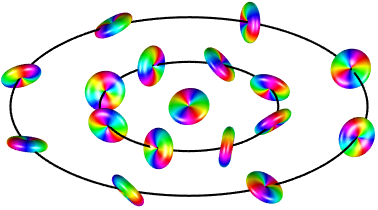
\includegraphics[width=\textwidth]
        {gfx/ch-spin2/C-FM=2_coreless_FM_init_spherical.pdf}
        \caption{\label{subfig: coreless-initial}}
    \end{subfigure}
    \begin{subfigure}{0.45\textwidth}
        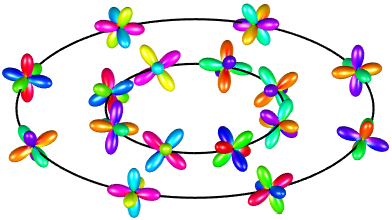
\includegraphics[width=\textwidth]
        {gfx/ch-spin2/C-FM=2_coreless_cyclic_init_spherical.pdf}
        \caption{\label{subfig: DQV-initial}}
    \end{subfigure}
    \caption{\label{fig: coreless-doubly-quantised} Spherical harmonic
        representation of the vortex configurations on each side of the FM-BN
        interface defined in Eq.~\eqref{eq: FM-BN-coreless-DQV}.
        (a): Spin-2 FM coreless vortex given by Eq.~\eqref{eq: FM-BN-coreless}.
        (b): Doubly quantised vortex on the BN side of the interface, given by
        Eq.~\eqref{eq: FM-BN-DQV}.
        \textcolor{red}{Current DQV is for cyclic case, update to BN.}}
\end{figure}
By tracing a point about the vortex line, the phase changes by a total of
\(4\pi \) indicating a doubly quantised vortex.

\subsection{Uniaxial nematic to biaxial nematic}\label{subsec: UN-BN-defects}
Consider \(D_1 \neq 0\) and \(D_2 = 0\), then \(\zeta_1 = \zeta_{-1} = 0\).
Furthermore, if \(\tilde{\mu} = \alpha \), then all of \(\zeta_{\pm 2}\) and
\(\zeta_0\) can be non-zero.
\textcolor{red}{Rest of derivation here.}

The final solution reads
\begin{equation}\label{eq: UN-BN-interpolating-spinor}
    \zeta_\mathrm{UN-BN} = \mqty(
    \frac{\sqrt{1 - \eta}}{2} \\
    0 \\
    \sqrt{\frac{1 + \eta}{2}} \\
    0 \\
    \frac{\sqrt{1 - \eta}}{2}
    ),
\end{equation}
where \(\eta = 10q /|c_2|n \in [-1, 1]\).
This solution depends only on the quadratic Zeeman shift, which can alter the
spinor between phases.
When \(q = c_2n / 10\) the system is in the uniaxial nematic phase.
In the opposite limit when \(q = -c_2n/10\) the system is in the biaxial
nematic phase.
This spinor therefore provides interpolating solutions between the uniaxial
nematic and biaxial nematic phases, engineered through manipulation of the
quadratic Zeeman shift.

To determine the stability of this interpolating spinor, we compare the energy
per particle given by~\cite{Kawaguchi2012}
\begin{equation}
    E_\mathrm{part} = \sum_{m=-2}^{2}(-pm + qm^2)|\zeta_m|^2 + \frac{c_0n}{2}
    + \frac{c_1n}{2}|\vb{f}|^2 + \frac{c_2n}{2}|a_{00}|^2.
\end{equation}
The energy of the interpolating spinor given in
Eq.~\eqref{eq: UN-BN-interpolating-spinor} reads
\(E^\mathrm{UN-BN}_\mathrm{part} = 2q + c_0n/2 - 10q^2/c_2n\)
\textcolor{red}{Messy notation}.
Comparing this energy with that of the UN phase
\(E^\mathrm{UN}_\mathrm{part} = (c_0+c_2/5)n/2\) reveals that this interface is
stable for \(|q| \leq |c_2|n/10\).

The consequence of a spatially-dependent \(\eta \) is revealed from the spin
singlet-duo and -trio amplitudes.
Upon substitution of Eq.~\eqref{eq: UN-BN-interpolating-spinor} into
\textcolor{red}{Define duo and trio amplitudes, more than likely in theory
    chapter} yields
\begin{equation}
    \begin{aligned}
        |A_{20}|^2 & = \frac{1}{10} \left[(\eta^2-1)\cos\theta
        + \eta^2 + 1\right],                                          \\
        |A_{30}|^2 & = \frac{1+\eta}{4} \left[3\left(\eta ^2-1\right)
            \cos\theta
            + \eta(5 \eta -8) + 5\right],
    \end{aligned}
\end{equation}
where \(\theta = \chi_2 + \chi_{-2} - 2\chi_0\) and \(\chi_j = Arg(\psi_j)\) for
component \(j=-2, 0, 2\).
We plot both the singlet-duo and -trio amplitudes in
Fig.~\ref{fig: UN-BN-duo-trio} in a parameter space of \((\eta, \theta)\).
\begin{figure}
    \centering
    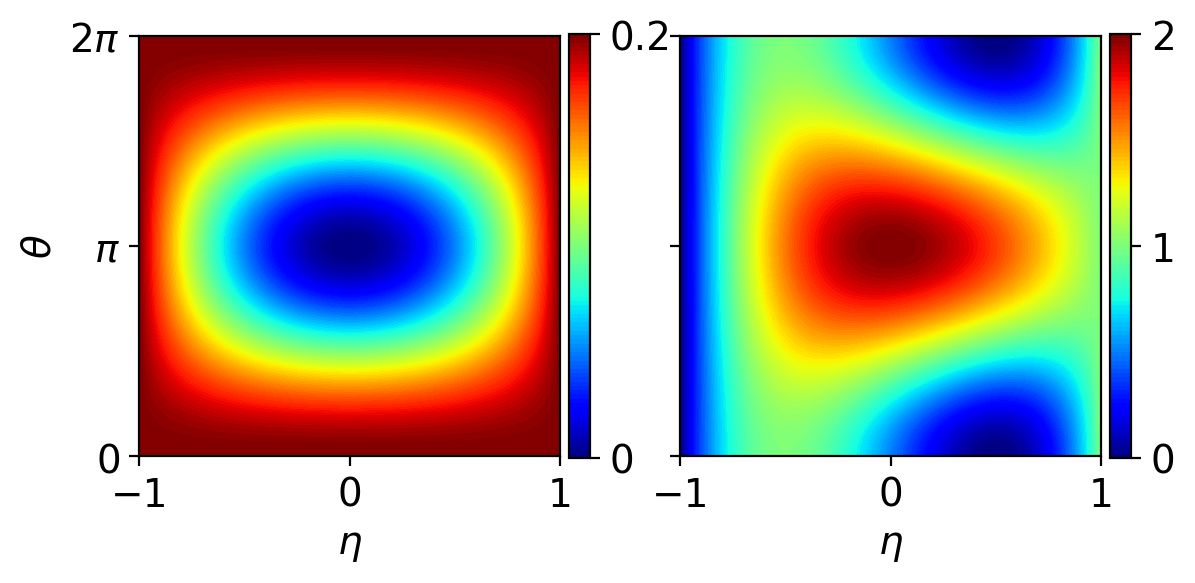
\includegraphics[width=0.75\textwidth]{gfx/ch-spin2/a20-a30-varying.png}
    \caption{\label{fig: UN-BN-duo-trio} Spin singlet-duo (left) and -trio
        (right) amplitudes for the interpolating spinor in
        Eq.~\eqref{eq: UN-BN-interpolating-spinor}.
        Due to the spatially-dependent \(\eta \), this spinor continuously
        interpolates between the UN, BN, and cyclic phases depending on the
        relative phase difference between the components.}
\end{figure}
We see that this spinor interpolates between the different phases of UN, BN and
cyclic depending on both \(\eta \) and the relative phase difference
\(\theta \).
For example, if one were to maintain \(\theta=0\) and interpolate \(\eta \),
then there would be multiple transitions between the UN (\(|a_{00}|^2 = 1\)) and
BN (\(|a_{00}|^2 = 0\)) phases.
As we shall see in the numerical investigation of such an interface, this has
profound effects on the structure of topological defects connecting across
the interface.

From the interpolating spinor in Eq.~\eqref{eq: UN-BN-interpolating-spinor} we
can construct various topological defect crossing solutions.
The simplest case is the connection of SQVs on either side of the interface.
Such a connection is realised by the choice \(\phi = \varphi \) whilst keeping
the Euler angles constant.
A representative example with \(\alpha = \gamma = 0\) is given by
\begin{equation}
    \zeta^\mathrm{SQV}_\mathrm{UN-BN} =
    \frac{e^{i\varphi}}{8}\begin{pmatrix}
        \sqrt{6} D_+ \sin ^2\beta _0 + 2D_- \left(\cos^2\beta _0+1\right) \\
        -2 \left(D_--\sqrt{3} D_+\right) \sin 2 \beta _0                  \\
        \sqrt{2}\left[ \sqrt{3} D_- \sin ^2\beta _0 -2D_+
        \left(1-3 \cos^2 \beta _0\right)\right]                           \\
        2 \left(D_--\sqrt{3} D_+\right) \sin 2 \beta _0                   \\
        \sqrt{6} D_+ \sin ^2\beta _0+D_- \left(\cos^2\beta _0+1\right)
    \end{pmatrix},
    \label{eq: UN-BN-SQV-SQV}
\end{equation}
where \(D_{\pm} = \sqrt{1 \pm \eta}\) and \(\beta=\beta_0\) is an arbitrary
constant.
The explicit form of the above equation in the UN
(\(D_+ = \sqrt{2}, D_- = 0\)) and BN (\(D_0 = 0, D_- = \sqrt{2}\)) limits
is given, respectively, as
\begin{equation}
    \zeta_\mathrm{UN}^\mathrm{SQV} =  \frac{e^{i\varphi}}{4}\mqty(
    \sqrt{3}\sin^2\beta_0 \\
    \sqrt{6}\sin2\beta_0 \\
    -2(1 - 3\cos^2\beta_0) \\
    -\sqrt{6}\sin2\beta_0 \\
    \sqrt{3}\sin^2\beta_0
    ), \qquad
    \zeta_\mathrm{BN}^\mathrm{SQV} =  \frac{e^{i\varphi}}{4}\mqty(
    \sqrt{2}(\cos^2\beta_0 + 1) \\
    -\sqrt{2}\sin2\beta_0 \\
    2\sqrt{3}\sin^2\beta_0 \\
    \sqrt{2}\sin2\beta_0 \\
    \sqrt{2}(\cos^2\beta_0 + 1)
    ).
\end{equation}
One can see that upon the substitution of \(\beta_0 = 0\) in the above spinors,
we recover the SQV case in both the UN
\(\zeta^\mathrm{SQV} = {(0,0,e^{i\varphi},0,0)}^T\) and BN
\(\zeta^\mathrm{SQV} = {(e^{i\varphi},0,0,0,e^{i\varphi})}^T/\sqrt{2}\) limits.
It is important to note that, despite being characterised by the same phase
winding, the SQVs on either side of the interface represent entirely different
objects due to the differing topologies of the UN and BN phases.

Spin vortices can be connected across the interface by choosing
\(\alpha=\varphi, \beta=\beta_0 \) and \(\phi = \gamma = 0\), resulting in the
spinor
\begin{equation}\label{eq: UN-BN-SV-SV-spinor}
    \zeta^\mathrm{SV} =
    \frac{1}{8}\begin{pmatrix}
        e^{-2i\varphi}\left[\sqrt{6} D_+ \sin ^2\beta _0
        + 2D_- \left(\cos^2\beta _0+1\right)\right]                   \\
        -2e^{-i\varphi} \left(D_--\sqrt{3} D_+\right) \sin 2 \beta _0 \\
        \sqrt{2}\left[ \sqrt{3} D_- \sin ^2\beta _0
        - 2D_+ \left(1-3 \cos^2 \beta _0\right)\right]                \\
        2 e^{i\varphi}\left(D_--\sqrt{3} D_+\right) \sin 2 \beta _0   \\
        e^{2i\varphi}\left[\sqrt{6} D_+ \sin ^2\beta _0
            + 2D_- \left(\cos^2\beta _0+1\right)\right]
    \end{pmatrix}.
\end{equation}
In particular, spin vortices arise in both components for
\(\beta_0 \neq 0, \pi \), where the spin vortex in each phase carries opposite
the spin winding of the other spin vortex.
For the specific cases of \(\beta_0 = 0, \pi \),
Eq.~\eqref{eq: UN-BN-SV-SV-spinor} instead results in a spin vortex in the BN
phase that continuously connects to a vortex-free state in the UN limit.

In addition to line defects, i.e., vortices, it is also possible to construct
point defects that terminate at the topological interface.
The possibility in the UN-BN interface is that of a monopole, which is
characterised by a spherically symmetric dependence of the nematic axis
\(\vb{\hat{d}} = (\cos\varphi \sin\theta, \sin\varphi \sin\theta, \cos\theta)\),
where \(\theta \) is the polar angle in spherical coordinates.
The monopole solution is derived from Eq.~\eqref{eq: UN-BN-interpolating-spinor}
using the substitution \(\beta = \theta \) and \(\alpha=\varphi \).
\textcolor{red}{Would quite like an image of the initial state somehow.}


\subsection{Cyclic to nematic}
A steady-state solution that interpolates between the nematic and cyclic phases
can be found by including phase coefficients in
Eq.~\eqref{eq: UN-BN-interpolating-spinor}, namely
\begin{equation}\label{eq: C-N-interpolating-spinor}
    \zeta^\mathrm{C-N} = \mqty(
    e^{i\chi_2}\frac{\sqrt{1 + \eta}}{2} \\
    0 \\
    e^{i\chi_0}\sqrt{\frac{1 - \eta}{2}} \\
    0 \\
    e^{i\chi_{-2}}\frac{\sqrt{1 + \eta}}{2}),
\end{equation}
where \(\eta = 10q/(|c_2|n)\).
The quadratic Zeeman shift can be used to interpolate the above solution between
the different phases.
At \(q = 0\) the above solution becomes the three component cyclic
\(\zeta_\mathrm{C} = {(1, 0, i\sqrt{2}, 0, 1)}^T/2\).
The sign of the quadratic Zeeman shift determines which nematic state is chosen.
If \(q = -c_2n/10\) then the solution becomes biaxial nematic
\(\zeta_\mathrm{BN} = {(1, 0, 0, 0, 1)}^T/\sqrt{2}\).
In the opposite limit of \(q = c_2n/10\) then the system is in the uniaxial
nematic state \(\zeta_\mathrm{UN} = {(0, 0, 1, 0, 0)}^T\).

One can construct all the defect states considered in the UN-BN interface
using this interpolating spinor between the cyclic and nematic phases.
To do so, we simply replace \(D_+ \rightarrow iD_+\) in
Eq.~\eqref{eq: UN-BN-SQV-SQV}, where the cyclic limit is identified as
\(D_+=D_-=1\).
In addition to those states, one can construct \textcolor{red}{Integer spin
    vortices?}

\subsection{Cyclic to ferromagnetic}
An additional stationary solution can be found by considering \(D_1=D_2=0\).
Eq.~\eqref{eq: D2} and Eq.~\eqref{eq: D1} can then be solved exactly, to yield
\begin{equation}
    \tilde{\mu} = \pm \sqrt{4q^2 + |\alpha|^2}.
\end{equation}
If \(q \neq 0\), then \(\tilde{\mu} \neq \alpha \) which implies \(\zeta_0=0\)
from Eq.~\eqref{eq: spin-2-stationary-zeta0-recast}.
Zero transverse magnetisation then implies we have
\(0 = 2c_1n(\zeta_2^*\zeta_{1} + \zeta_{-1}^*\zeta_{-2})\).
\textcolor{red}{Rest of derivation here.}

The final solution reads
\begin{equation}\label{eq: C-FM-interpolating-spinor}
    \zeta^\mathrm{C-FM} = \frac{1}{\sqrt{3}}\mqty(
    \sqrt{1 + f_z} \\
    0 \\
    0 \\
    \sqrt{2 - f_z} \\
    0
    ),
\end{equation}
where \(f_z = (p - q) / (c_1n)\) gives the \(z\)-component of the spin vector.
At zero magnetisation, \(f_z = 0\), this solution is precisely the two-component
cyclic state.
The solution also interpolates between different ferromagnetic states depending
on the value of the magnetisation.
If \(f_z = -1\) one recovers an FM-1 solution
\(\zeta_\text{FM-1} = {(0, 0, 0, 1, 0)}^T\).
Conversely, \(f_z = 2\) yields the FM-2 solution
\(\zeta_\text{FM-2} = {(1, 0, 0, 0, 0)}^T\).
This spinor therefore provides a family of interpolating solutions between the
cyclic and both ferromagnetic phases.

Applying a phase and a general spin rotation to the spinor in
Eq.~\eqref{eq: C-FM-interpolating-spinor} yields (\(\beta = 0\))
\begin{equation}\label{eq: C-FM-general-spinor}
    \zeta^\text{C-FM} = \frac{e^{i\varphi}}{\sqrt{3}}\mqty(
    e^{-2i(\alpha+\gamma)}D_2 \\
    0 \\
    0 \\
    e^{i(\alpha+\gamma)}D_{-1} \\
    0
    ),
\end{equation}
where \(D_2 = \sqrt{1 + f_z}\) and
\(D_{-1} = \sqrt{2 - f_z}\).
Now, combinations of \(\phi \) and \(\alpha+\gamma \) yields different phase
vortices.
Since the cyclic phase supports fractional vortices
(see Sec. \textcolor{red}{Section}), we are able to construct a myriad of
different connections from this interpolating spinor.
For example, the choice \(\alpha+\gamma=-\varphi/3\) and \(\phi=\varphi/3\)
results in a singular SQV in the FM-2 limit (\(D_2 = 1, D_{-1} = 0\)),
a third vortex in the cyclic limit (\(D_2 = \sqrt{1/3}, D_{-1} = \sqrt{2/3}\)),
and a vortex-free state in the FM-1 limit (\(D_2 = 0, D_{-1} = 1\)).
Instead, by choosing \(\alpha + \gamma = \varphi/3\) and \(\phi = 2\varphi/3\)
we have a vortex-free state in the FM-2 limit, a two-third vortex in the cyclic
limit, and a singular SQV in the FM-1 limit.
A case constructing SQVs in all three limits is given by \(\alpha+\gamma = 0\)
and \(\phi = \varphi \).

One can use the general spinor in Eq.~\eqref{eq: C-FM-general-spinor} to
analytically examine the vortex core structures when \(D_{2,{-1}}\) are
functions of the transverse radius \(\rho = \sqrt{x^2 + y^2}\).
The states can be described by choosing an appropriate function for
\(f_z(\rho)\) that interpolates between all three phases.
We choose \(f_z(\rho) = 3\tanh(\rho/2) - 1\) which becomes \(f_z=-1\) at
\(\rho=0\), \(f_z=0\) and hence cyclic at \(\rho=\tanh^{-1}(1/3)\), and
finally \(f_z=2\) at large \(\rho \).
The resulting spin magnitude and singlet-trio amplitude using the above
substitution in Eq.~\eqref{eq: C-FM-general-spinor} are plotted in
Fig.~\ref{fig: C-FM-analytical-spin-singlet}.
\begin{figure}
    \centering
    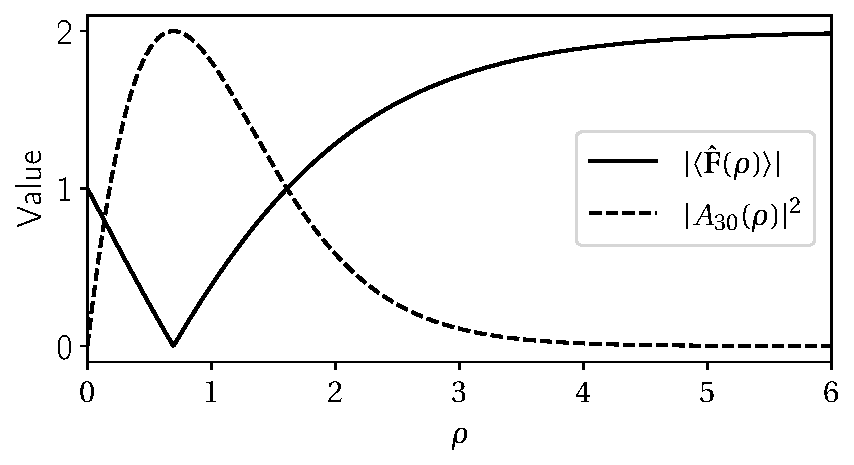
\includegraphics[width=0.5\textwidth]
    {gfx/ch-spin2/spin_singlet_radius_analytical.pdf}
    \caption{\label{fig: C-FM-analytical-spin-singlet}
        Analytical calculation of the spin magnitude (solid line) and
        spin-singlet trio amplitude (dashed line) using the initial state in
        Eq.~\eqref{eq: C-FM-interpolating-spinor}.
        We choose \(f_z(\rho) = 3\tanh(\rho/2) - 1\) to mode all three phases of
        this interpolating spinor.
        \textcolor{red}{Plot takes up a lot of space. Can I pair it with
            something?}
    }
\end{figure}
\textcolor{red}{Need to expand this discussion and really get my head around
    what this plot shows in relation to a vortex.}

In addition to phase vortices, we can construct a coreless vortex in the FM
phase that connects to a vortex state in the cyclic phase.
To construct the characteristic fountain-like spin texture, we choose a
monotonically increasing function of \(\beta=\beta(\rho)\).
The order-parameter is then kept single-valued by a combined winding of the
condensate phase coupled to a winding of the spin vector, achieved by
\(\phi'=2\alpha=2\varphi \), where \(\phi'=\phi-2\gamma \).
Applying such a rotation to the general spinor in
Eq.~\eqref{eq: C-FM-interpolating-spinor} yields
\begin{equation}\label{eq: C-FM-coreless-general}
    \zeta^\text{cl} = \frac{1}{\sqrt{3}}\left(D_2\zeta^\text{|F|=2}_\text{cl}
    + D_{-1}\zeta^\text{|F|=1}_\text{cl}\right),
\end{equation}
where
\begin{equation}\label{eq: C-FM-coreless-FM-limits}
    \zeta^{|F|=2}_\text{cl} =
    \mqty(
    \cos^4\frac{\beta}{2} \\
    2e^{i\varphi}\cos^3\frac{\beta}{2}\sin\frac{\beta}{2} \\
    \sqrt{6}e^{2i\varphi}\cos^2\frac{\beta}{2}\sin^2\frac{\beta}{2} \\
    2e^{3i\varphi}\cos\frac{\beta}{2}\sin^3\frac{\beta}{2} \\
    e^{4i\varphi}\sin^4\frac{\beta}{2}
    ), \qquad
    \zeta^{|F|=1}_\text{cl} =
    \mqty(
    -\cos\frac{\beta}{2}\sin^3\frac{\beta}{2} \\
    e^{i\varphi}\sin^2\frac{\beta}{2}\left(\cos^2\frac{\beta}{2}
    -\sin^2\frac{\beta}{2}\right) \\
    -\sqrt{\frac{3}{8}}e^{2i\varphi}\sin2\beta \\
    e^{3i\varphi}\cos^2\frac{\beta}{2}\left(\cos^2\frac{\beta}{2}
    -3\sin^2\frac{\beta}{2}\right) \\
    2e^{4i\varphi}\cos^3\frac{\beta}{2}\sin\frac{\beta}{2}
    )
\end{equation}
represent coreless vortices in both the FM-2 and FM-1 limits, respectively.
The spherical harmonic representation of these coreless vortices are shown
in Fig.~\ref{subfig: C-FM-FM2-coreless},~\ref{subfig: C-FM-FM1-coreless}.
\begin{figure}
    \centering
    \begin{subfigure}{0.49\textwidth}
        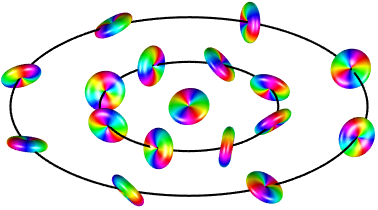
\includegraphics[width=\textwidth]
        {gfx/ch-spin2/C-FM=2_coreless_FM_init_spherical.pdf}
        \caption{\label{subfig: C-FM-FM2-coreless}}
    \end{subfigure}
    \begin{subfigure}{0.49\textwidth}
        \includegraphics[width=\textwidth]{example-image-b}
        \caption{\label{subfig: C-FM-FM1-coreless}}
    \end{subfigure}\\
    \begin{subfigure}{0.49\textwidth}
        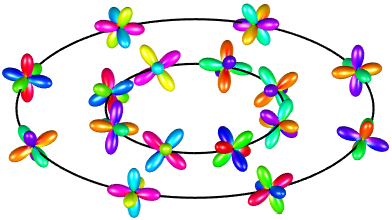
\includegraphics[width=\textwidth]
        {gfx/ch-spin2/C-FM=2_coreless_cyclic_init_spherical.pdf}
        \caption{\label{subfig: C-FM-cyclic-DQV}}
    \end{subfigure}
    \caption{\label{fig: C-FM-coreless-initial-states}Spherical harmonic
        representation of the interface in Eq.~\eqref{eq: C-FM-coreless-general}.
        (a) and (b): Coreless vortex in the FM-2 and FM-1 limit, respectively,
        given by Eq.~\eqref{eq: C-FM-coreless-FM-limits}.
        (c): Doubly quantised vortex in the cyclic limit, given by
        Eq.~\eqref{eq: C-FM-DQV-cyclic-limit}.}
\end{figure}
The resulting spinor in the cyclic limit is
\begin{equation}\label{eq: C-FM-DQV-cyclic-limit}
    \zeta^\text{DQV}
    = \left(\zeta^\text{|F|=2}_\text{cl}
    + \sqrt{2}\zeta^\text{|F|=1}_\text{cl}\right) / 3.
\end{equation}
The spherical harmonic representation of this cyclic state is plotted in
Fig.~\ref{subfig: C-FM-cyclic-DQV}.
By tracing a point about the vortex core, the condensate phase winds by a total
of \(4\pi \), indicating that this is a doubly-quantised vortex.

\section{Numerical investigations of defect crossing physics}
In this section we numerically investigate some topological interfaces defined
in the preceding section, along with a subset of the possible defect
connections.

Our numerical setup is as follows.
We numerically evolve the spin-2 GPEs defined in
Eqs.~\eqref{eq: spin-2-GPEs-pm2} -~\eqref{eq: spin-2-GPEs-0} using a symplectic
integrator~\cite{SymesNumeric2017} using a purely isotropic trapping potential
\(V=M\omega^2r^2/2\).
We simulate the energy loss during experiments by introducing a phenomenological
damping coefficient, \(\gamma \), through the substitution
\(t \rightarrow (1-i\gamma)t\).
In all simulations considered, we choose \(\gamma = 1e-2\).
We perform our simulations on a 3D of \(N_s^3=128^3\) points, with side lengths
\(L = 20\ell \), where \({(\ell =\hbar/M\omega)}^{1/2}\) is the (isotropic)
harmonic oscillator length.
We choose parameters that correspond to a \(^{87}\)Rb
condensate~\cite{Klausen2001} with \(c_0n=1.32\times10^4\hbar\omega\ell^3\),
\(c_0/c_1=90.7\), and \(c_0/c_2=-102\), where the ground state is predicted to
be nematic.
In each simulation, we perform a small spin rotation to the initial state to
avoid components that are identically zero.
Additionally, when constructing states with defects, the position of each defect
is perturbed slightly to avoid artificial stability when placed at exactly the
centre of the trap.


\subsection{Uniaxial nematic to biaxial nematic interface}
The first interface we consider is that between the UN and BN phases, considered
in Sec.~\ref{subsec: UN-BN-defects}.
Since the UN and BN phases are energetically degenerate in the absence of a
magnetic field, we introduce a spatially-dependent quadratic Zeeman shift
\(q(z)\) such that \(q(z) > 0\) on the UN side and \(q(z) < 0\) on the BN side,
to lift the degeneracy.
The quadratic Zeeman shift linearly interpolates over a small transition region,
which we take to be small compared to the spin-dependent healing lengths.

Our investigation begins with that of the SQV-SQV connection, where the initial
state is constructed as in Eq.~\eqref{eq: UN-BN-SQV-SQV} with \(\beta_0=0\).
To imprint the vortices, we perform a short imaginary time propagation, then
proceed to numerically evolve the spin-2 GPEs.

The dynamics of this connection is split into two distinct parts.
Firstly, upon evolution, the two overlapping SQVs spatially separate due to an
instability occurring at the interface \(z \approx 0\).
Each SQV then connects to a vortex-free state on the other side of the
interface (\textcolor{red}{Figure showing this potentially}).

After the initial separation, the cores of the vortices fill with atoms
occupying different ground states, drastically altering the order parameter
symmetry within the cores (see Fig.~\ref{fig: UN-BN-SQV-SQV-singlets}).
\begin{figure}
    \centering
    \begin{subfigure}{0.33\textwidth}
        \includegraphics[width=\textwidth]{example-image}
        \caption{Spatial separation.}
    \end{subfigure}
    \begin{subfigure}{0.33\textwidth}
        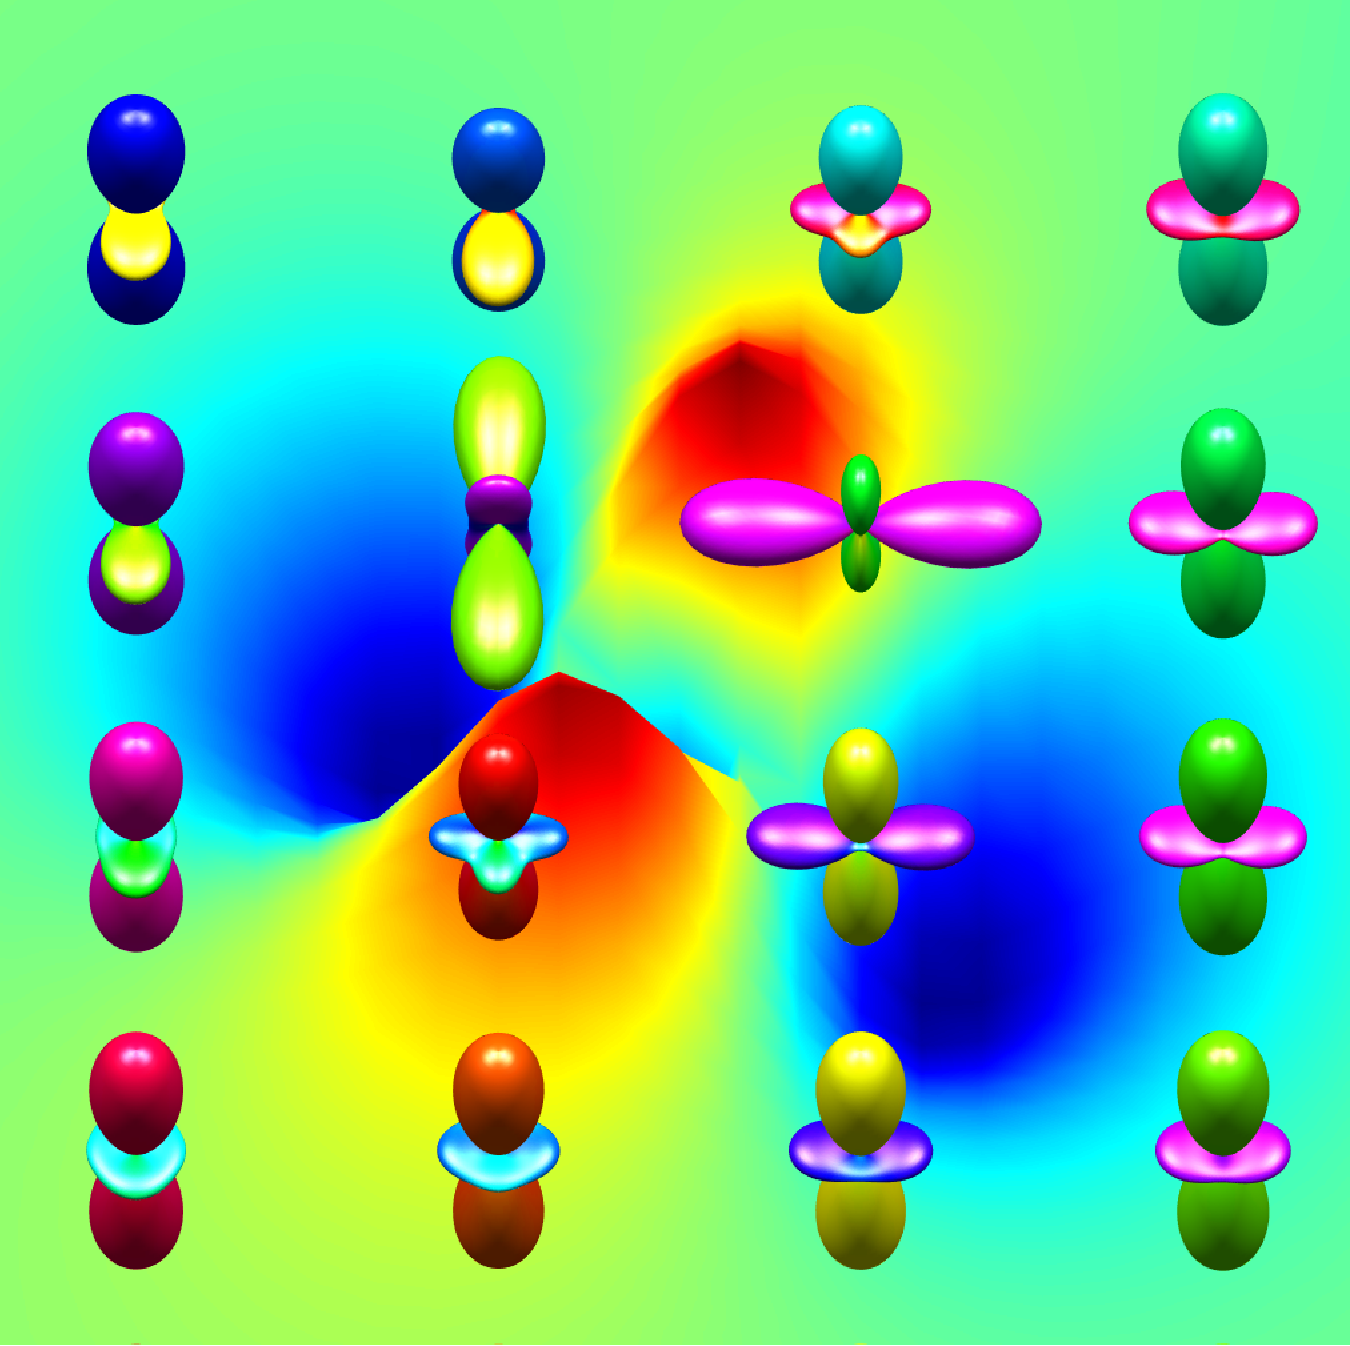
\includegraphics[width=\textwidth]
        {gfx/ch-spin2/UN-BN_SQV-SQV_singletTrio_UN.png}
        \caption{}
    \end{subfigure}
    \begin{subfigure}{0.33\textwidth}
        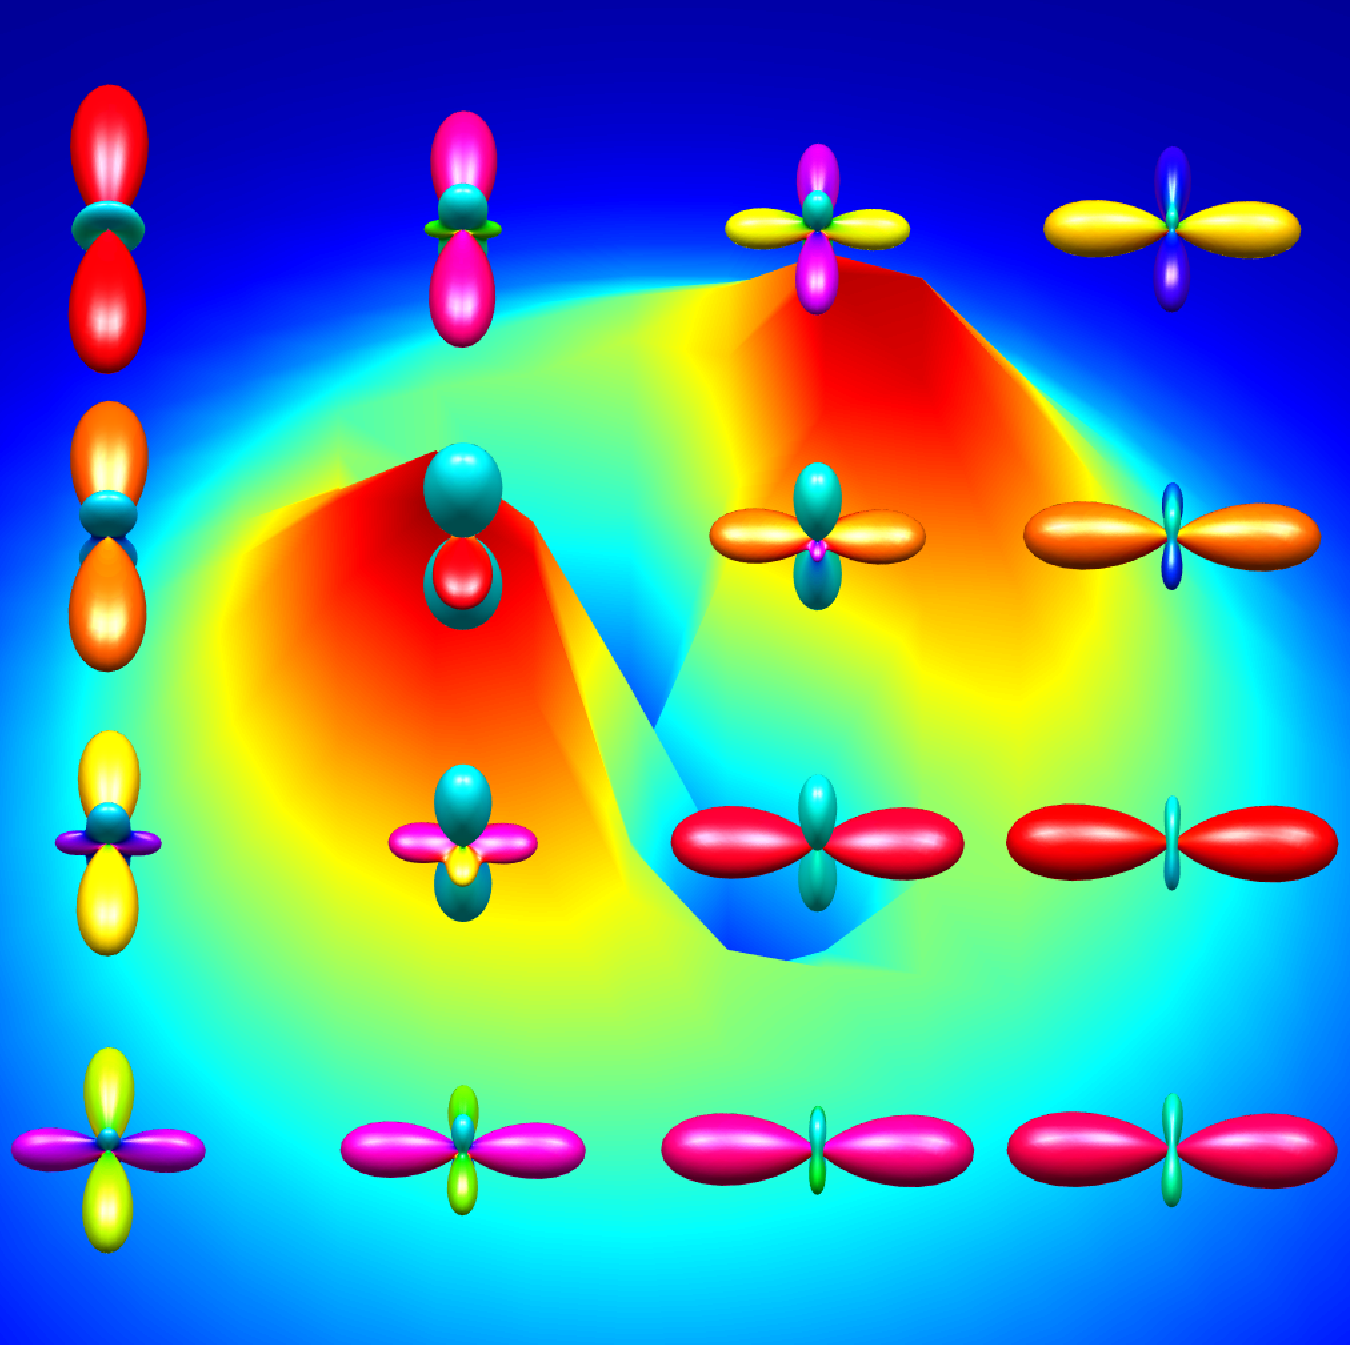
\includegraphics[width=\textwidth]
        {gfx/ch-spin2/UN-BN_SQV-SQV_singletTrio_BN.png}
        \caption{}
    \end{subfigure}\\
    \begin{subfigure}{0.33\textwidth}
        \includegraphics[width=\textwidth]{example-image}
        \caption{Plot showing FM regions.}
    \end{subfigure}
    \begin{subfigure}{0.33\textwidth}
        \includegraphics[width=\textwidth]{example-image}
        \caption{Pure imaginary time plot showing SQV splitting on BN side.}
    \end{subfigure}
    \begin{subfigure}{0.33\textwidth}
        \includegraphics[width=\textwidth]{example-image}
        \caption{Maybe not needed.}
    \end{subfigure}
    \caption{\label{fig: UN-BN-SQV-SQV-singlets}Transverse cuts of
    \(|A_{30}|^2\) for the SQV-SQV connection given in
    Eq.~\eqref{eq: UN-BN-SQV-SQV} at \(\bar{t} = 300\) on the UN (a) and BN (b)
    sides of the interface.
    Overlaid are the spherical harmonics showing the non-trivial change of the
    order parameter symmetry.}
\end{figure}
In the UN case, the initially empty core fills with atoms occupying both the
cyclic and BN phases, generating a topological interface within the core itself.
This likely arises due to the differing phases factors between the wave function
components, as seen in Fig.~\ref{fig: UN-BN-duo-trio}.

The SQV on the BN undergoes a similar filling of the empty vortex core.
This time, the core fills with atoms in the UN, FM, and cyclic phases, also
generating an interface within the core.
The outer UN core is occupied by two small FM regions with
\(|\langle \hat{F} \rangle| = 2\), in addition to a larger, central cyclic
region \textcolor{red}{Plots highlighting the FM regions, hard to see from
    current plot}.
Spherical harmonics constructed about the core reveal that the phase winds by
\(\pi \) about these FM regions, accompanied by a \(\pi/2\) rotation of the
condensate spin vector.
The development of this composite core structure signifies the start of a
splitting process, whereby the SQV is expected to split into two HQVs.
Since our system has no rotation to stabilise the vortices, the timescales
considered here reveal that both vortices eventually leave the condensate
cloud.
Additionally, the SQV on the BN side of the interface will leave the condensate
before the splitting into two HQVs has occurred.
However, Fig.~\textcolor{red}{relevant fig} shows a purely imaginary time
simulation of the initial state in Eq.~\eqref{eq: UN-BN-SQV-SQV} with
\(\beta_0 = 0\) showing the resulting HQVs after the initial SQV has split.

We next investigate the spin vortex connection, using the initial state in
Eq.~\eqref{eq: UN-BN-SV-SV-spinor} with \(\beta_0=0\).
\textcolor{red}{Need to do simulation of this. May or may not include,
    depending on result.}

We can also investigate a vortex connection that terminates on the interface.
We start with the initial state in Eq.~\eqref{eq: UN-BN-SQV-SQV} with
\(\beta_0=0\), and artificially remove the winding from the middle component.
The result is a SQV in the BN phase that smoothly connects to a vortex-free
state in the UN phase.
The resulting spin magnitude and singlet-trio amplitude after purely
imaginary-time relaxation are plotted in Fig.~\ref{fig: UN-BN-VF-SQV}.
\begin{figure}
    \centering
    \begin{subfigure}{0.33\textwidth}
        \includegraphics[width=\textwidth]{example-image}
        \caption{}
    \end{subfigure}
    \begin{subfigure}{0.33\textwidth}
        \includegraphics[width=\textwidth]{example-image}
        \caption{}
    \end{subfigure}
    \begin{subfigure}{0.33\textwidth}
        \includegraphics[width=\textwidth]{example-image}
        \caption{}
    \end{subfigure}
    \caption{\label{fig: UN-BN-VF-SQV} UN-BN VF-SQV plots go here.}
\end{figure}
The dynamics of this connection closely resembles what the later dynamics of the
BN side of the SQV-SQV connection would look like, provided that the vortices
were stabilised against leaving the condensate.
We see that the initial SQV on the BN side has undergone a splitting process
into two HQVs, each of which terminate at the interface.
The cores of the HQVs are easily identified from the
\(|\langle \hat{\vb{F}} \rangle = 2\) regions.
Similar splitting of an SQV into HQVs has been observed in the polar phase of
spin-1 condensates~\cite{Seo2015, Xiao2021}.
For the timescales considered, the resulting HQVs remain stable against
leaving the condensate.

\textcolor{red}{Monopole?}

\subsection{Cyclic to ferromagnetic interface}
We numerically investigate vortex connections across a topological interface
between the cyclic and FM-2 phases, given by
Eq.~\eqref{eq: C-FM-interpolating-spinor}.
Since our numerical simulations use parameters that predict a nematic ground
state, we introduce a spatially-dependent \(c_1\) term such that \(c0/c_1=90.7\)
on the cyclic side but \(c_0/c_1=-90.7\) on the FM side, effectively changing
the sign of the \(c_1\) term.
Now, in the FM region, the parameters ensure that the FM region remains stable.
Despite the cyclic state not being the predicted ground state, the interface
is observed to remain stable for the timescales considered in our simulations.

We firstly investigate the connection of a third vortex in the cyclic phase
connecting to a singular SQV in the FM-2 phase using
Eq.~\eqref{eq: C-FM-general-spinor} with \(\alpha + \gamma = \varphi/3\) and
\(\phi=\varphi/3\) as the initial state.
The initial state is then propagated using a short imaginary-time evolution to
imprint the vortex cores.
From here we switch to complex-time using a damping coefficient of
\(\gamma=10^{-2}\).

The resulting spin magnitude is plotted in Fig.~\ref{fig: C-FM-third-SQV} where
non-trivial core structures emerge.
\begin{figure}
    \centering
    \begin{tikzpicture}
        \node[inner sep=0pt] (plot0) at (-2,0)
        {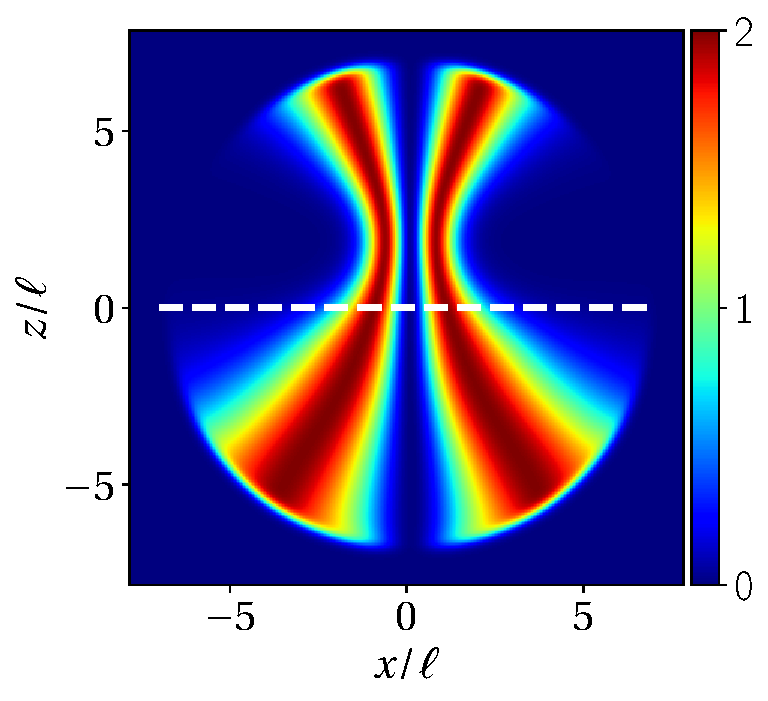
\includegraphics[width=0.33\textwidth]
            {gfx/ch-spin2/C-FM=2_third-SQV_singlet_duo.pdf}};
        \node[inner sep=0pt] (plot1) at (0,0)
        {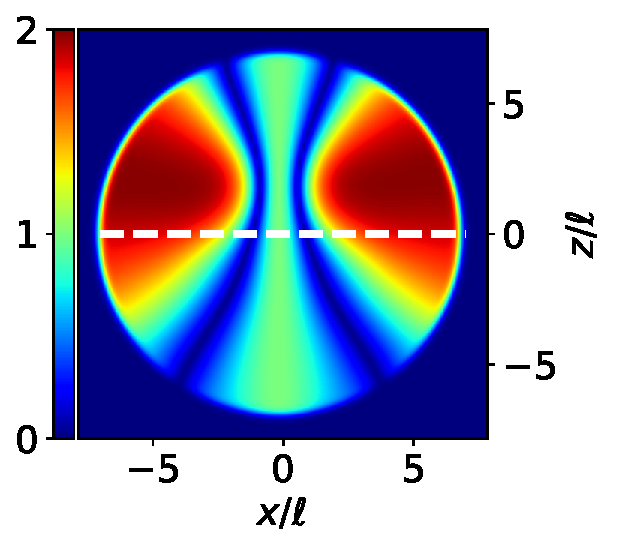
\includegraphics[width=0.33\textwidth]
            {gfx/ch-spin2/C-FM=2_third-SQV_spinMag.pdf}};
        \node[inner sep=0pt] (plot2) at (4, 0)
        {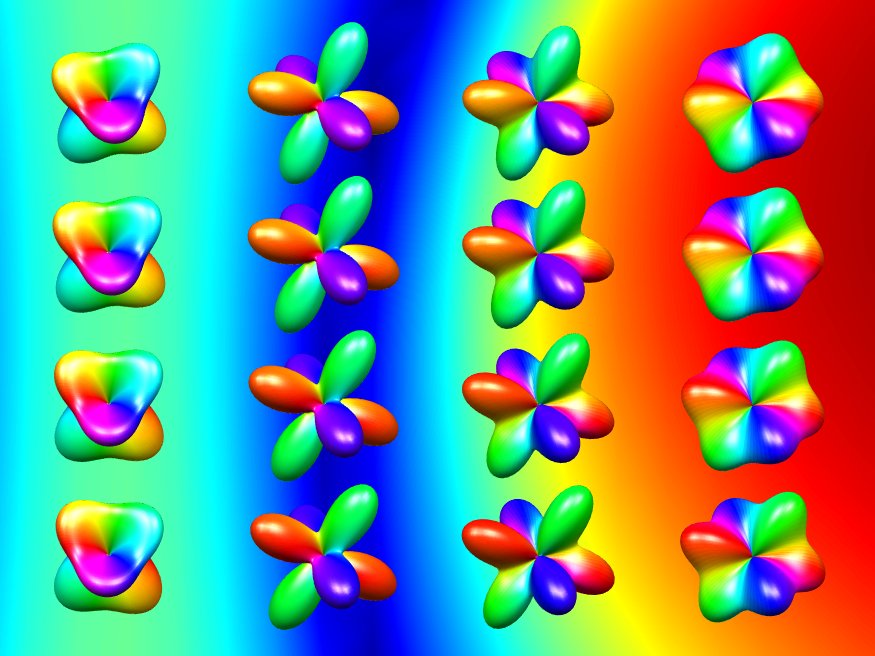
\includegraphics[width=0.3\textwidth, height=0.3\textwidth]
            {gfx/ch-spin2/C-FM=2_third-SQV_spinMag_spherical.pdf}};
        \node[rectangle, draw=black, minimum width=0.5cm, minimum height=0.5cm]
        (rec) at (0, 0.75) {};
        \draw[-, dashed] (rec.north west) -- (plot2.north west) {};
        \draw[-, dashed] (rec.south west) -- (plot2.south west) {};

        \draw[-, thick] (plot2.south east) -- (plot2.north east) {};
        \draw[-, thick] (plot2.south east) -- (plot2.south west) {};
        \draw[-, thick] (plot2.south west) -- (plot2.north west) {};
        \draw[-, thick] (plot2.north west) -- (plot2.north east) {};
    \end{tikzpicture}
    \caption{\label{fig: C-FM-third-SQV}\textcolor{red}{\(|A_{20}|^2\) plot
    too.}}
\end{figure}

\subsection{Cyclic to biaxial nematic interface}
